\documentclass{article}

%================  CUSTOMIZATION  =================================================%

\usepackage{../KjelsethReportStyle}

%================  METADATA  ======================================================%

\title{\fontsize{24}{36}\selectfont Elektroniske enheter og kretser\\ % Input title
Lab 01} % Line 2 of title, \\ means next line.

\author{{\ttfamily Sølve Kjelseth}} % Input your name.
% replace \ttfamily with \normalfont to make it regular font.
% (removing \ttfamily will not do this automatically.

\date{\today} % Auto updates the date, untill you export it.


%================  START OF DOCUMENT  =============================================%

\begin{document}

\maketitle % Makes title front page based on the title, author and date metadata, change at the top

%================  SECTION  =======================================================%

\addtocontents{toc}{\protect\setcounter{tocdepth}{0}} % Temporarily hide from TOC
\section{Introduction} % Numbered section named Introduction
This is the first report in this course, detailing the completion of the first lab exercise.\par
\vfill
Note: As always, the \LaTeX\ file and all other assets, such as text, images, graphs and code made by me for this project is open source with the MIT licence, see
\linkgithub[true][0.5]{my GitHub}

\clearpage

%================  SECTION  =======================================================%

\tableofcontents % Generate TOC
\hfill
\listoffigures % List of figures
\hfill
\listoftables % List of tables
\addtocontents{toc}{\protect\setcounter{tocdepth}{2}} % Restore TOC depth

%================  SECTION  =======================================================%

\section{Part 1 - Diode test}
This Part is about testing a diode charachteristics with a multimeter. This means it is inherently not perfect, but it will function as a reference measurment.

%================  SINGLE FIGURE  =================================================%

\begin{figure}[h]
    \centering
    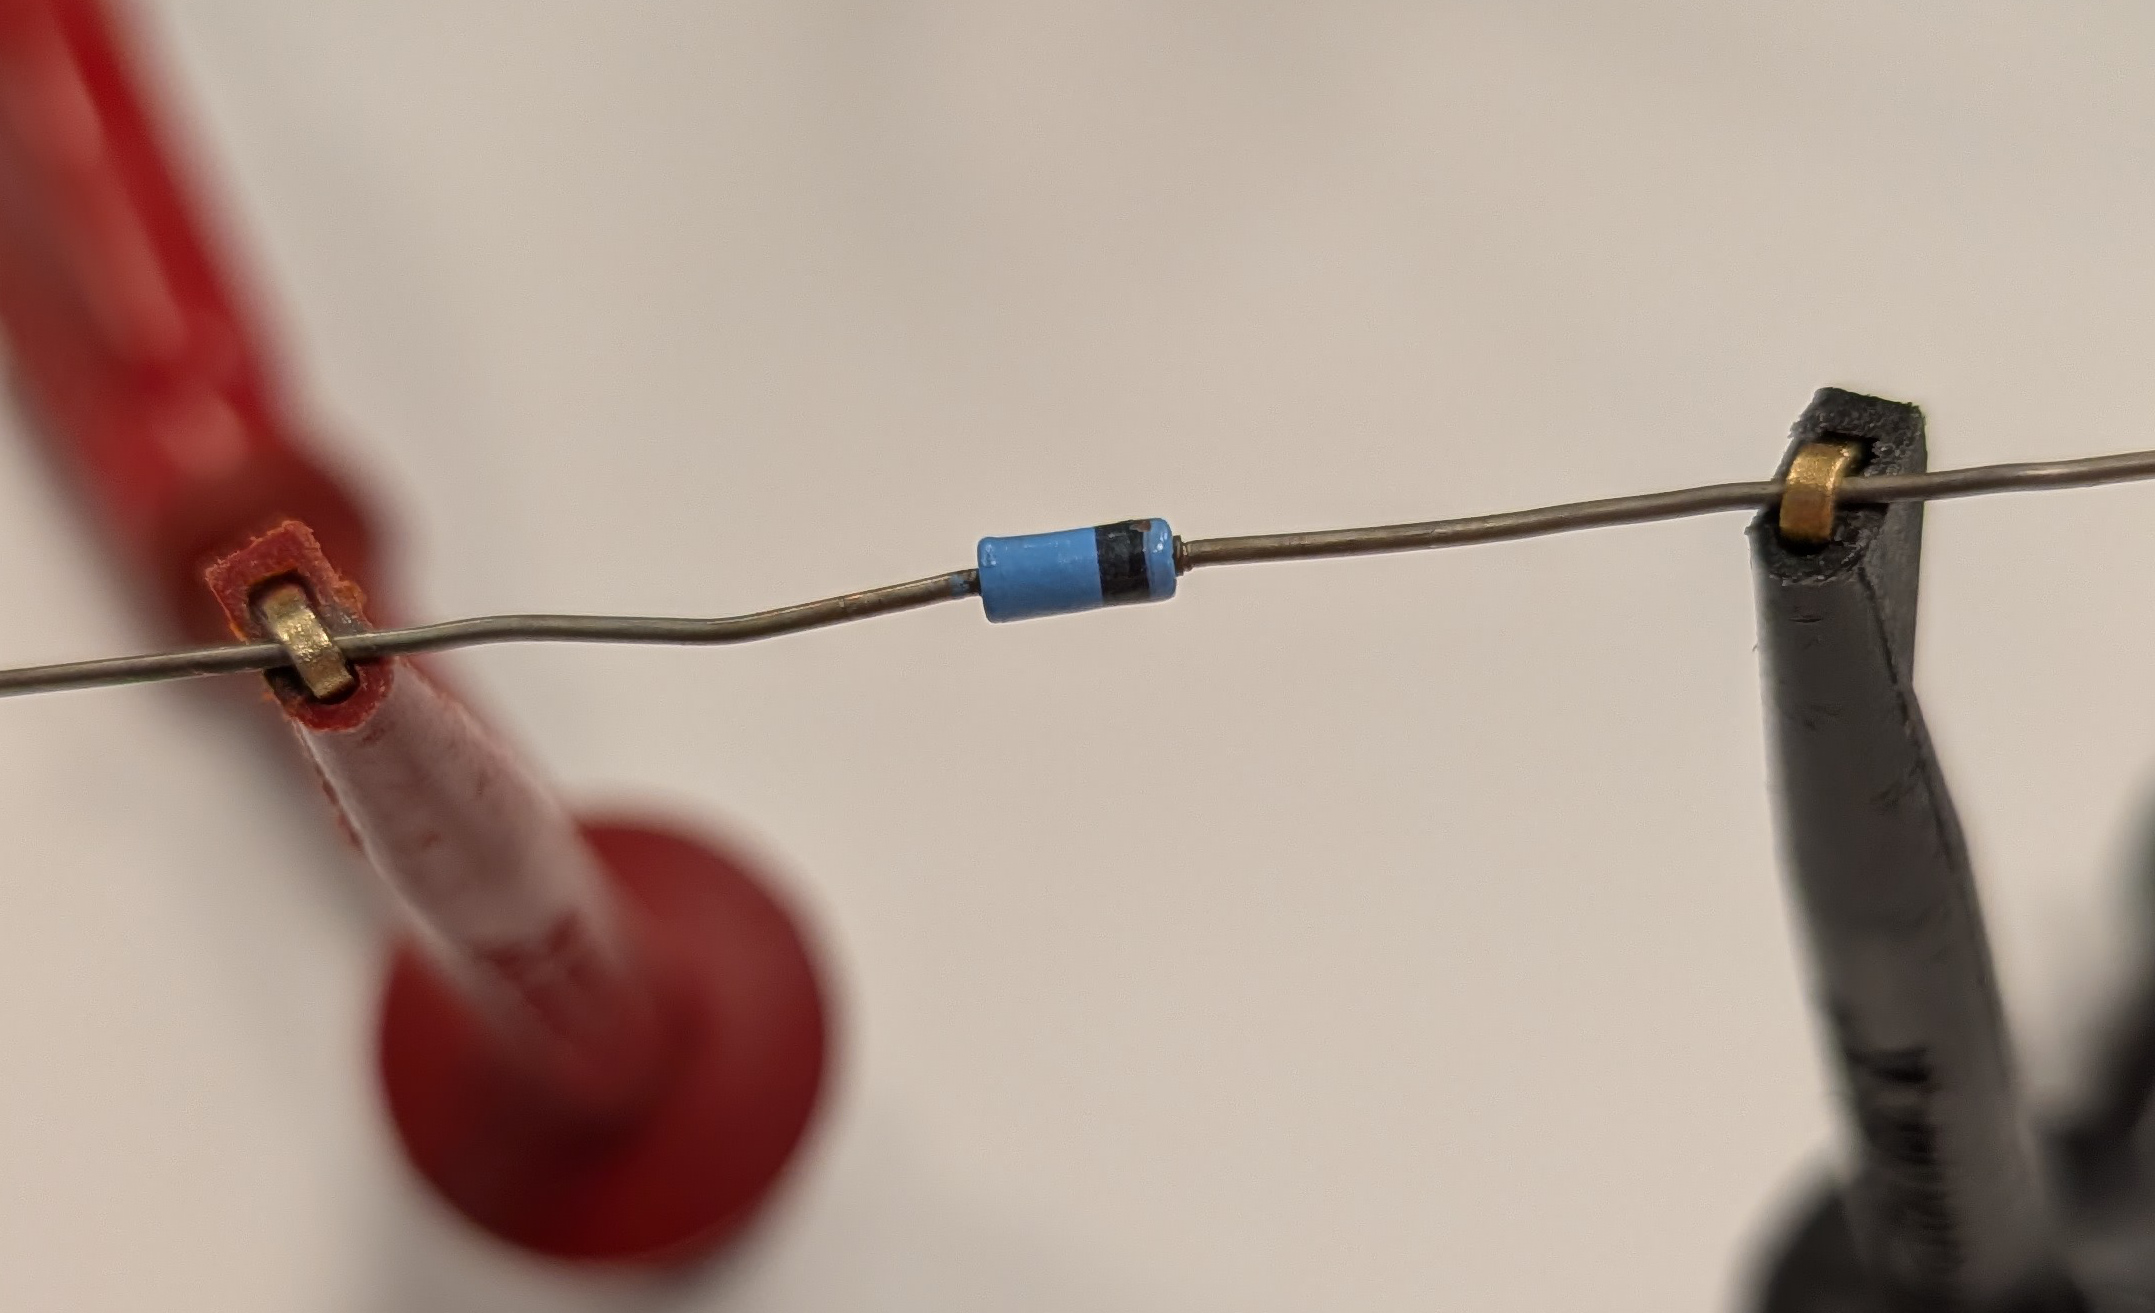
\includegraphics[width=0.8\textwidth]{Part1.jpg}
    \caption{Diode being measured}
    \label{fig:part1}
\end{figure}

%================  TABLE  =========================================================%

% Table generated by Excel2LaTeX from sheet 'Sheet1'
\begin{table}[htbp]
  \centering
  \caption{Diode measurments}
    \begin{tabular}{|l|lr|l|lr|}
    \hline
    Voltage forward & \multicolumn{1}{r}{0.593} & \multicolumn{1}{l|}{V} & Resistance forward & \multicolumn{1}{r}{225400} & \multicolumn{1}{l|}{\Omega} \bigstrut\\
    \hline
    Voltage reverse & OL    &       & Resistance reverse & OL    &  \bigstrut\\
    \hline
    \end{tabular}%
  \label{tab:part1}%
\end{table}%

%================  SECTION  =======================================================%

\section{Part 2 - Forward-bias charachteristics}
This Part is about testing the diode charachteristics for forward-bias. The values was stored in a table (RAW data like this is found on the \linkgithub{GitHub}) and then a plot was made to compare the current through the diode \(I_D\) with the voltage drop over the diode \(V_D\).

%================  SINGLE FIGURE  =================================================%

\begin{figure}[h]
    \centering
    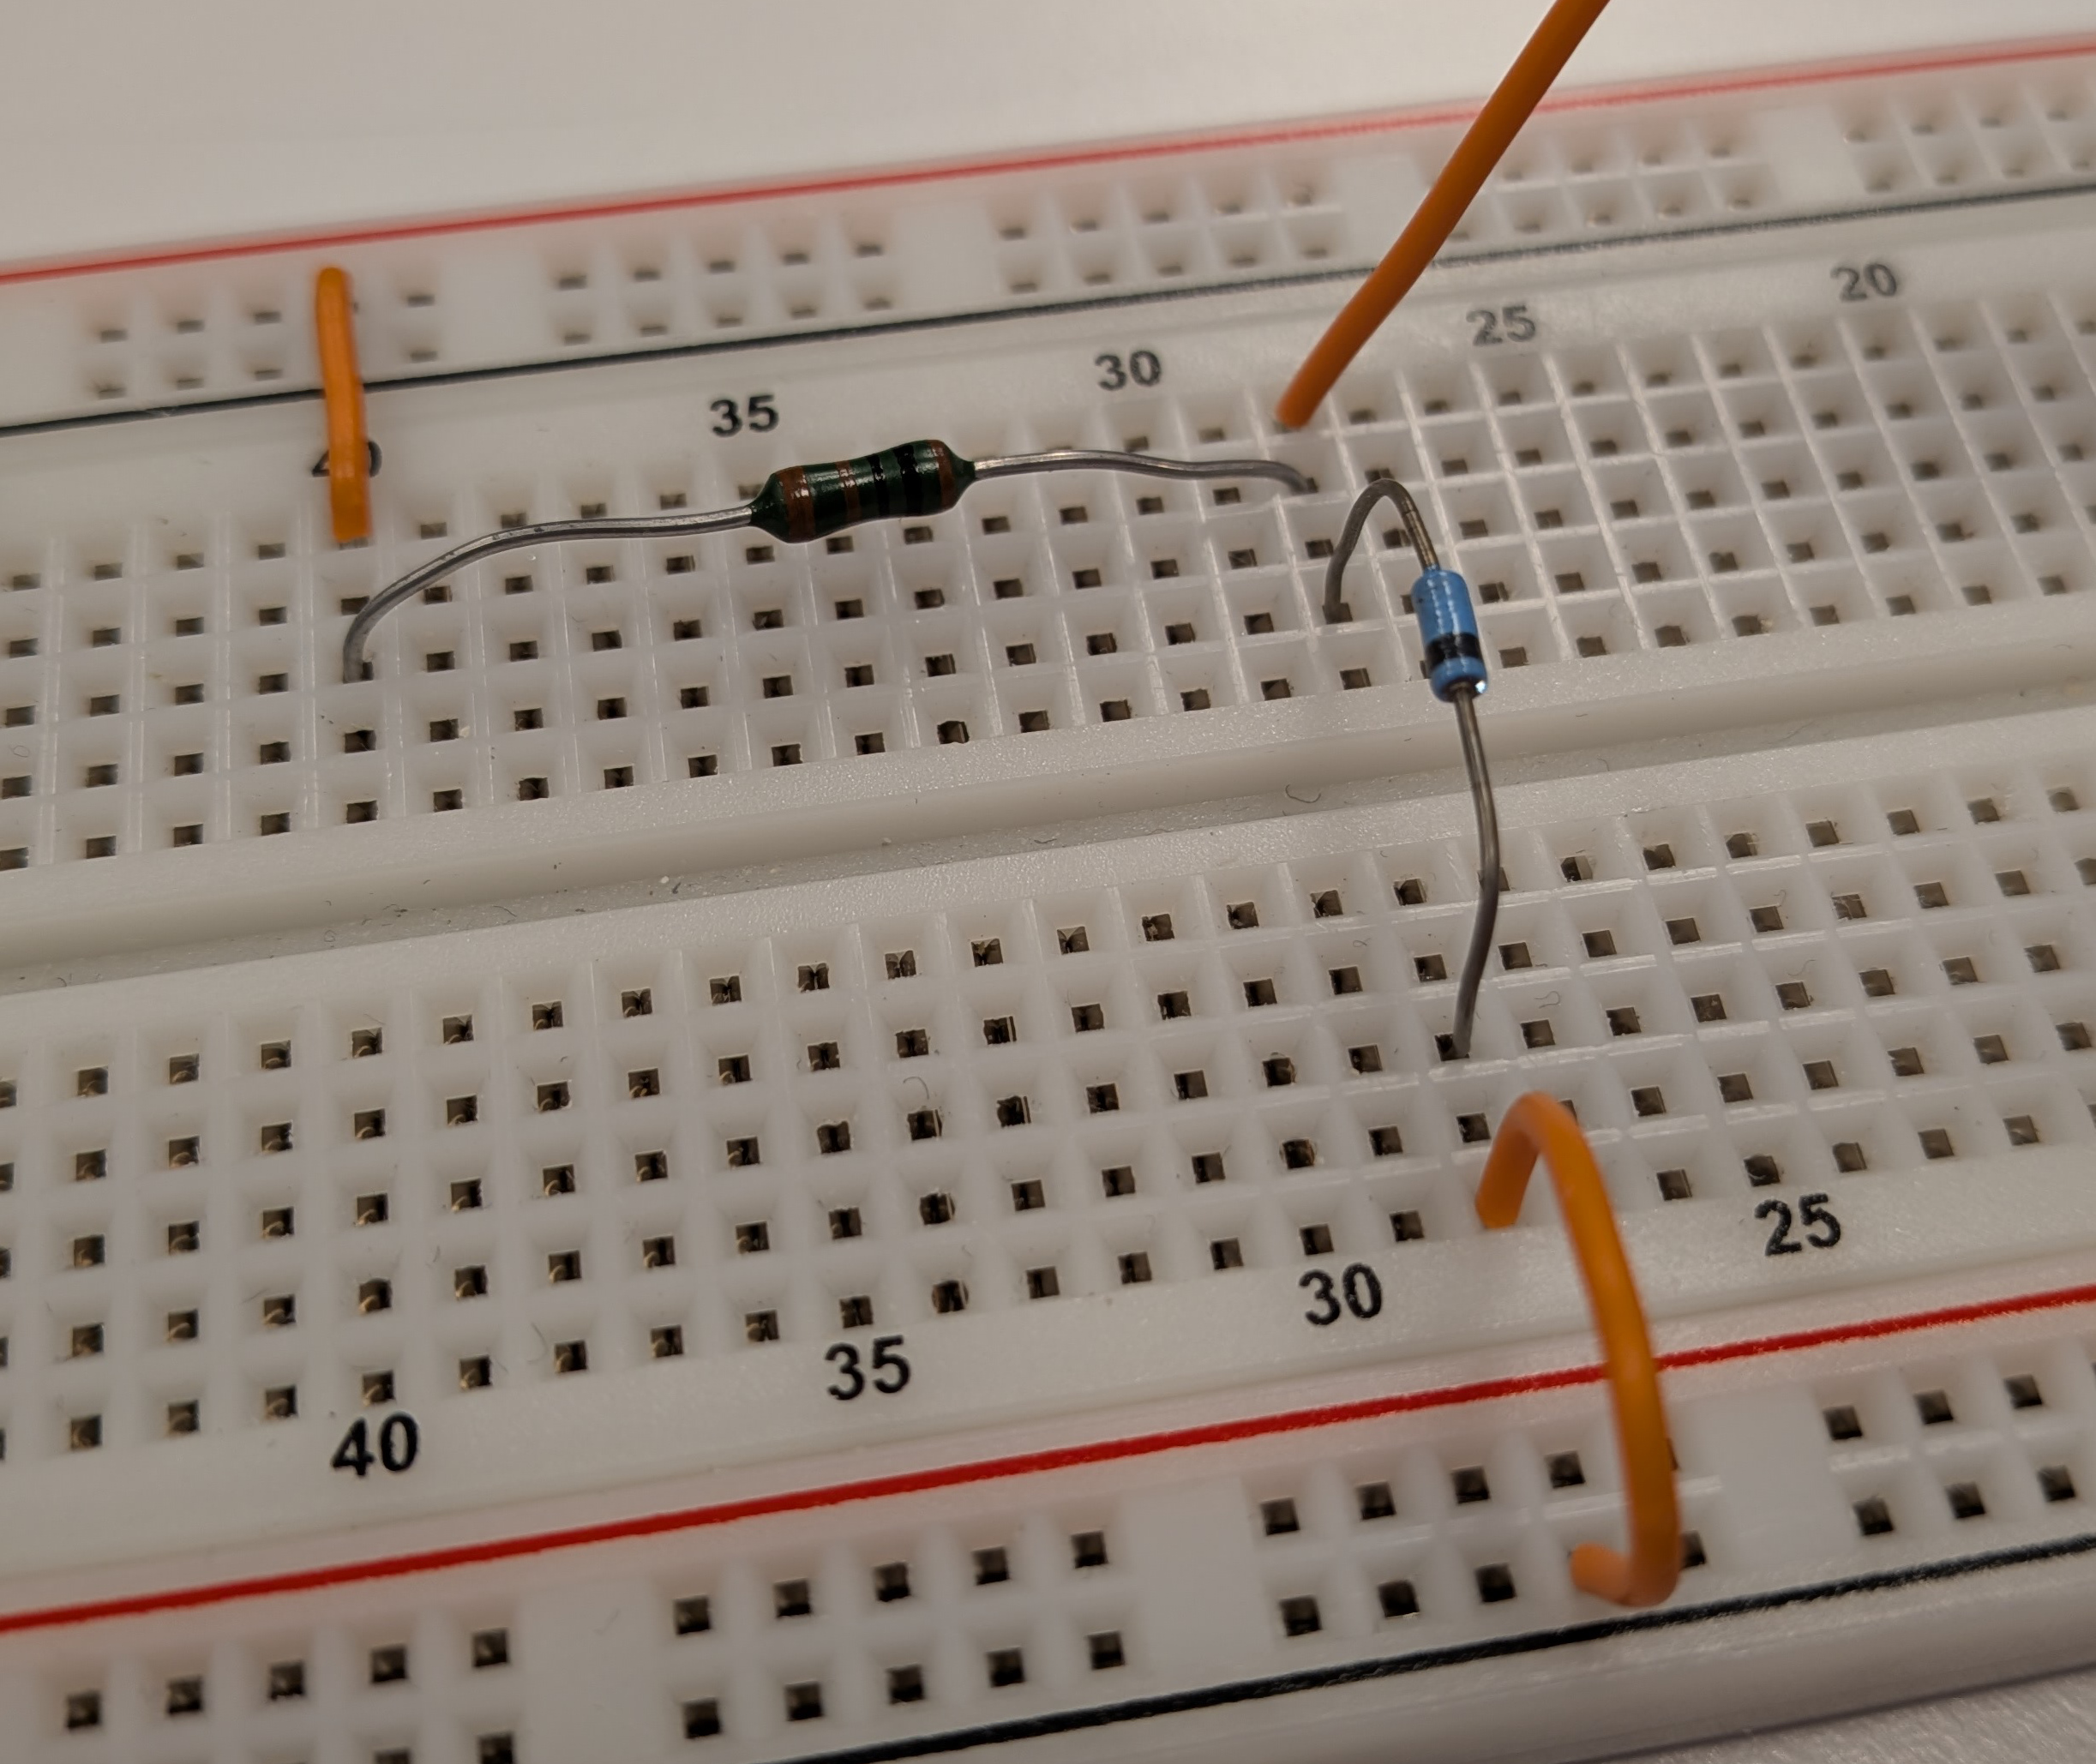
\includegraphics[width=0.8\textwidth]{Part2.jpg}
    \caption{Part 2 circuit}
    \label{fig:Part2}
\end{figure}

\clearpage

%================  SINGLE FIGURE  =================================================%

\begin{figure}[h]
    \centering
    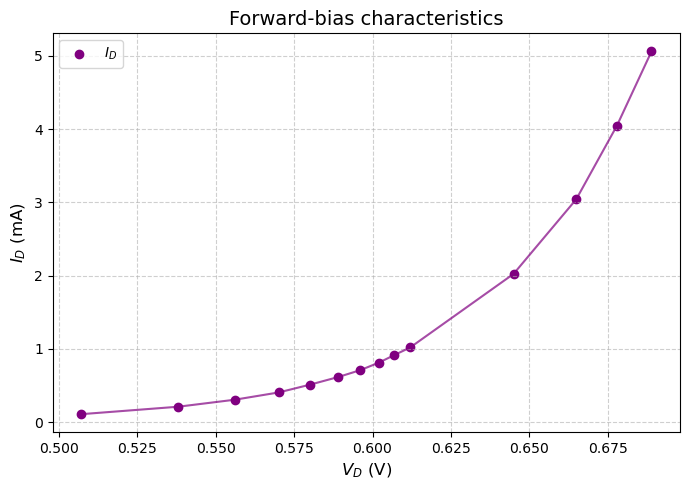
\includegraphics[width=\textwidth]{Part2Plot.png}
    \caption{Plot of forward-bias charachteristics}
    \label{fig:Part2Plot}
\end{figure}

\end{document}